% 第17章第5节：指派与带权二部图匹配（指派问题；可行标号与紧边证书；KM算法及矩形、不完整配对；Auction算法及误差缩放；方法比较与结果检验）。

\section{指派与带权二部图匹配}
\label{sec:graph-assignment}

上一节只关心能配上多少对。若每名员工都必须分到一项任务、不同配对花费不同，就要在全部完整配对中挑总成本最低的一个。逐人挑最便宜的任务会让几个人挤向同一项任务，所以需要判断“谁让出偏爱的任务更划算”，并证明得到的方案已经最省。

给每名员工和每项任务各配一个数，可以得到任何完整配对成本的下界；只用恰好达到下界的边完成的配对就是最优的。KM算法保持下界有效，在这些边上用交替路径扩大匹配，受阻时抬高下界；Auction算法让员工为任务出价，用价格协调争抢，得到误差可控的方案。

\subsection{指派问题}
\label{sec:graph-opt-assign-problem}

把员工看成二部图左侧的行，任务看成右侧的列。行$i$与列$j$允许配对时，两者之间有一条边，成本$c_{i,j}$是有限实数，可以为负；不允许的配对没有边。

\begin{definition}[指派问题]
\label{def:graph-opt-assignment}
设二部图两侧各有$r$个顶点，左侧为行$1,\ldots,r$，右侧为列$1,\ldots,r$，允许的行列对组成边集$E$，每条边$(i,j)\in E$有有限实成本$c_{i,j}$。\term{指派问题}（assignment problem）要求选出一个只用允许边的完美匹配，即给每行$i$指定一个不同的列$\sigma(i)$，使总成本$C(\sigma)=\sum_{i=1}^r c_{i,\sigma(i)}$最小。
\end{definition}

指派问题也称为最小权完美匹配，输出一个最优指派，或“不存在完美匹配”的结论。若要使收益$w_{i,j}$之和最大，取$c_{i,j}=-w_{i,j}$即可。全部行列对都允许时，$\sigma$可以是任意置换，成本写成$r$阶矩阵$\bm C=(c_{i,j})$。

“每个顶点恰配一次”不能随意放宽。允许匹配任意多对、只求收益最大的是另一个问题，即最大权匹配：负收益的边宁可不选，结果可能只配一部分顶点；在最小成本形式下，成本全为正时空匹配反而“最便宜”。行列数不等、禁配、可以不配但要付惩罚等情形，在第~\ref{sec:graph-opt-assign-rectangular}节归结为本定义；下文先在方阵上讲算法。

\subsection{可行标号与最优性条件}
\label{sec:graph-opt-assign-labels}

判断一个指派是否最优，不能把$r!$个指派逐一比较，需要一个能对全部指派同时成立的下界。给每行$i$配实数$u_i$，每列$j$配实数$v_j$。若对每条允许边都有
\begin{equation}
  u_i+v_j\leq c_{i,j},
  \label{eq:graph-opt-feasible-labels}
\end{equation}
就称$(\bm u,\bm v)$为\term{可行标号}（feasible labeling）：把成本分摊给行与列，两份之和不超过实际成本。对任意完整指派$\sigma$，把它用到的$r$条边的不等式相加；每行恰出现一次，每列也恰出现一次，于是
\[
  C(\sigma)=\sum_{i=1}^r c_{i,\sigma(i)}\geq\sum_{i=1}^r\bigl(u_i+v_{\sigma(i)}\bigr)=\sum_{i=1}^r u_i+\sum_{j=1}^r v_j.
\]
右边与$\sigma$无关，是全部完整指派成本的共同下界。这个论证只用到“每行每列恰计一次”，不需要一般的线性规划对偶理论。

称$c_{i,j}-u_i-v_j\geq0$为边$(i,j)$的剩余量。剩余量为零、使式~\eqref{eq:graph-opt-feasible-labels}取等号的允许边称为\term{紧边}（tight edge），全部顶点与全部紧边组成的子图称为\term{相等子图}（equality subgraph）。
\begin{theorem}[紧边指派的最优性]
\label{thm:graph-opt-tight-assignment}
设$(\bm u,\bm v)$是可行标号。若完整指派$\sigma$只使用紧边，即$\sigma$是相等子图中的完美匹配，则$C(\sigma)=\sum_iu_i+\sum_jv_j$，因而$\sigma$是最优指派。
\end{theorem}

\begin{proof}
$\sigma$用到的每条边都取等号，上面的求和不等式也取等号，所以$\sigma$的成本等于下界。任何完整指派的成本都不低于这个下界，所以$\sigma$最优。
\end{proof}

可行标号本身只提供下界；相等子图里可能没有完美匹配，不能据此宣布最优。求解因此变成两件同时进行的事：保持标号可行，同时在紧边中凑出完美匹配。KM算法严格按此工作；Auction算法允许所选的边留下一点剩余量，误差在第~\ref{sec:graph-opt-auction}节给出。

\subsection{KM算法}
\label{sec:graph-opt-hungarian}

\term{KM算法}（Kuhn--Munkres algorithm）以Kuhn和Munkres命名，英文文献通常称为Hungarian algorithm，即带权的匈牙利算法；上一节的匈牙利算法只求最大匹配，没有成本。它从可行标号和空匹配出发，只在紧边上寻找增广路径，受阻时调整标号产生新的紧边；各列的最小剩余量作为状态维护，使复杂度与实际操作一致。

\subsubsection{主要思想}

沿用上一节的两名员工甲、乙和两项任务$1$、$2$，现在每个配对都允许，但成本不同：
\[
  \bm C=\begin{bmatrix}1&2\\1&4\end{bmatrix},
\]
行依次为甲、乙，第$j$列是任务$j$。完整方案只有两个：甲—$1$、乙—$2$成本为$5$；甲—$2$、乙—$1$成本为$3$。两人最便宜的选择都是任务$1$，“每行选最小”拼不成指派；要比较的是让步的代价：甲改做任务$2$多花$1$，乙则多花$3$。

把上一小节的标号放回成本表。从每行最小值出发取$\bm u=(1,1)$、$\bm v=(0,0)$，标号可行，各格剩余量$c_{i,j}-u_i-v_j$为
\[
  \begin{bmatrix}0&1\\0&3\end{bmatrix}.
\]
零格就是紧边。两个零格都在第一列，相等子图暂时没有完美匹配。

让甲先占任务$1$，再从自由的乙出发找增广路径。乙沿紧边到任务$1$，任务$1$已归甲，于是转去问甲；甲除任务$1$外没有紧边，搜索受阻，如图~\ref{fig:graph-opt-km}(a)。要接到空闲的任务$2$，甲还差$1$、乙还差$3$，所以只把标号推进较小的差额$1$：甲、乙的标号各加$1$，使通往树外的剩余量减$1$；任务$1$的标号减$1$，使树内两条紧边保持为零。新标号为$\bm u=(2,2)$、$\bm v=(-1,0)$，甲到任务$2$变紧，得到增广路径乙—任务$1$—甲—任务$2$，如图~\ref{fig:graph-opt-km}(b)。翻转后甲做任务$2$、乙做任务$1$，成本为$3$，等于标号之和$2+2-1+0$，由定理~\ref{thm:graph-opt-tight-assignment}最优。成本表没有被改写，改变的只是下界的表示。

\begin{figure}[!htb]
  \centering
  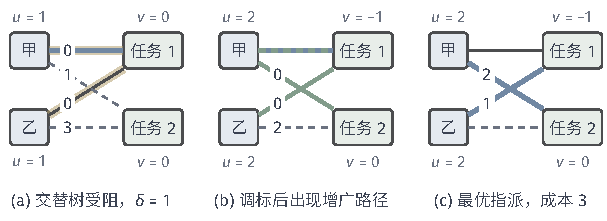
\includegraphics[width=102.799mm]{figures/01-basic-mathematics/04-graphs/tikz/c3-assign-km/figure.pdf}
  \caption{KM算法在成本矩阵$\left[\begin{smallmatrix}1&2\\1&4\end{smallmatrix}\right]$上的运行。顶点旁为标号，(a)(b)边旁为剩余量，(c)边旁为成本；实线为紧边，虚线为非紧边，粗蓝线为匹配。(a)从乙出发的交替树（黄色衬底）受阻，$\delta=1$。(b)调标后甲到任务$2$变紧，出现增广路径（绿色）。(c)指派成本$3$等于标号之和。}
  \label{fig:graph-opt-km}
\end{figure}

这个例子里的做法可以一般化。从一个自由行出发，只沿紧边生长\term{交替树}（alternating tree）：从行走未匹配的紧边到列，到达已匹配的列就沿匹配边回到它的行。记树中的行集为$S$、列集为$T$。到达自由列就沿树中路径增广；所有紧边都通向$T$时，在$S$到树外列的边中取最小剩余量$\delta$，令$S$中行标号加$\delta$、$T$中列标号减$\delta$。差额更大会违反式~\eqref{eq:graph-opt-feasible-labels}，更小则没有新的紧边。为了不在每次受阻时重新比较全部边，算法为每个树外列记住“从树中哪一行过来差得最少、差多少”\scite{math-graph-zeh-hungarian}。

\subsubsection{算法流程}

\paragraph{算法状态与初始化}
输入是允许边集与成本，运行中不变，不算状态。对照手算，算法维护以下状态：
\begin{itemize}
  \item 伙伴数组：每行配给的列、每列配给的行，初值全为空。
  \item 标号$\bm u,\bm v$：先检查每行至少有一条允许边，否则直接报告不可行；取$u_i=\min_{j:(i,j)\in E}c_{i,j}$，$v_j=0$。每条允许边满足$u_i+0\leq c_{i,j}$，标号可行，且每行至少有一条紧边。
  \item 交替树：行集$S$、列集$T$，以及每个入树列的前驱行，即把它带进树的那一行。为一个新的自由行建树时，$S$只含该行，$T$为空。
  \item 松弛量与来源：对每个树外列$j$，
  \[
    \mathrm{slack}(j)=\min\bigl\{c_{i,j}-u_i-v_j:\ i\in S,\ (i,j)\in E\bigr\},
  \]
  没有候选时记为$+\infty$；$\mathrm{from}(j)$记录取到最小值的行。建树时按根行的允许边初始化。
\end{itemize}
调标后交替树和来源记录都保留，只有增广成功后，才为下一个自由行重建这些状态。

\paragraph{扩树、调标与增广}
为一个自由行建树后，按情形反复执行：
\begin{itemize}
  \item 扩树：若有树外列$j$满足$\mathrm{slack}(j)=0$，就把$j$加入$T$，前驱记为$\mathrm{from}(j)$。若$j$已匹配，把它的行$i'$加入$S$，再只扫描$i'$的允许边，用$c_{i',j'}-u_{i'}-v_{j'}$更新各树外列的$\mathrm{slack}(j')$与$\mathrm{from}(j')$。
  \item 增广：若加入$T$的$j$是自由列，从$j$沿前驱和匹配边回溯到根，得到一条全由紧边组成的增广路径；翻转路径上的配对，匹配增加一对，本轮结束。
  \item 调标：若树外列的松弛量都为正，取
  \begin{equation}
    \delta=\min_{j\notin T}\mathrm{slack}(j),
    \label{eq:graph-opt-hungarian-delta}
  \end{equation}
  令$S$中各行$u_i\gets u_i+\delta$、$T$中各列$v_j\gets v_j-\delta$，各树外列$\mathrm{slack}(j)\gets\mathrm{slack}(j)-\delta$，来源不变。取到最小值的列松弛量变为零，随即可以扩树。
\end{itemize}
若需要调标时全部树外列的松弛量都为$+\infty$，报告不可行。全部行都匹配时停止，输出匹配与标号。

调标时行在$S$外、列在$T$中的边剩余量增加$\delta$，原来的紧边可能不再紧，相等子图并非只增不减；保留下来的是树中的边和匹配边，下一小节核对。

\begin{algorithm}[KM算法]
\label{alg:graph-opt-hungarian}
输入：两侧各$r$个顶点的允许边集与成本。输出：最优指派与可行标号，或“不可行”。
\begin{enumerate}
  \item 若某行没有允许边，报告不可行；否则置$u_i$为第$i$行最小允许成本、$v_j=0$，伙伴全为空。
  \item 若所有行都已匹配，转第6步。否则取自由行$i_0$，置$S=\{i_0\}$、$T=\varnothing$，对每列$j$置$\mathrm{slack}(j)=c_{i_0,j}-u_{i_0}-v_j$（不允许时为$+\infty$）、$\mathrm{from}(j)=i_0$。
  \item 若有$j\notin T$使$\mathrm{slack}(j)=0$：把$j$加入$T$，前驱置为$\mathrm{from}(j)$。若$j$自由，转第5步；否则把$j$的伙伴行$i'$加入$S$，对每个$j'\notin T$，若$c_{i',j'}-u_{i'}-v_{j'}<\mathrm{slack}(j')$，就更新$\mathrm{slack}(j')$并置$\mathrm{from}(j')=i'$；重复第3步。
  \item 若所有$j\notin T$都有$\mathrm{slack}(j)=+\infty$，报告不可行；否则按式~\eqref{eq:graph-opt-hungarian-delta}求$\delta$，$S$中行标号加$\delta$、$T$中列标号减$\delta$、树外列松弛量减$\delta$，回到第3步。
  \item 从自由列$j$开始，令$i$为$j$的前驱、$j''$为$i$原来的伙伴，把$i$改配给$j$，再令$j\gets j''$，直到$i=i_0$；回到第2步。
  \item 输出伙伴数组与标号$(\bm u,\bm v)$。
\end{enumerate}
\end{algorithm}

\paragraph{运行示例}
表~\ref{tab:graph-opt-hungarian-trace}把上面的手算翻译成状态：
\begin{itemize}
  \item 以甲为根，任务$1$的松弛量为$0$且空闲，直接增广，甲配任务$1$。
  \item 以乙为根，任务$1$入树；它已归甲，甲入树，只扫描甲的边，把任务$2$的松弛量从$3$（来自乙）降为$1$（来自甲）。
  \item 调标$\delta=1$，任务$2$的松弛量变为$0$，来源仍是甲。
  \item 任务$2$入树，前驱为甲；它空闲，回溯：甲改配任务$2$，任务$1$交给其前驱乙。
\end{itemize}
成本$3$等于标号之和，逐行贪心的成本$5$则不然。加入一行只扫描这一行、已有最小值继续保留，正是复杂度分析依赖的增量维护。

\begin{table*}[!htb]
  \centering\small
  \caption{KM算法在成本矩阵$\left[\begin{smallmatrix}1&2\\1&4\end{smallmatrix}\right]$上的状态。每行为动作后的状态；松弛量依次为任务$1$、$2$，括号内为来源，“—”表示已入树。}
  \label{tab:graph-opt-hungarian-trace}
  \begin{tabular}{@{}lllll@{}}
    \toprule
    动作 & $S$；$T$ & $\bm u$；$\bm v$ & 松弛量（来源） & 匹配 \\
    \midrule
    以甲为根建树 & $\{\text{甲}\}$；$\varnothing$ & $(1,1)$；$(0,0)$ & $0$（甲），$1$（甲） & 空 \\
    任务$1$入树，增广 & — & $(1,1)$；$(0,0)$ & — & 甲—$1$ \\
    以乙为根建树 & $\{\text{乙}\}$；$\varnothing$ & $(1,1)$；$(0,0)$ & $0$（乙），$3$（乙） & 甲—$1$ \\
    任务$1$、甲入树 & $\{\text{乙},\text{甲}\}$；$\{1\}$ & $(1,1)$；$(0,0)$ & —，$1$（甲） & 甲—$1$ \\
    调标$\delta=1$ & $\{\text{乙},\text{甲}\}$；$\{1\}$ & $(2,2)$；$(-1,0)$ & —，$0$（甲） & 甲—$1$ \\
    任务$2$入树，增广 & — & $(2,2)$；$(-1,0)$ & — & 甲—$2$，乙—$1$ \\
    \bottomrule
  \end{tabular}
\end{table*}

\subsubsection{正确性与复杂度}

两人例中下界从$2$升到$3$，与方案成本相等。一般情形依赖四件事：初始标号可行；扩树与调标保持标号可行、匹配紧和树中紧；调标后树能继续生长；每次增广增加一对。扩树和增广只沿紧边进行、不改标号，剩下的是调标。

\begin{lemma}[调标的效果]
设标号可行，匹配边与交替树中的边都是紧边，且$\delta$按式~\eqref{eq:graph-opt-hungarian-delta}取有限值。调标后标号仍可行，匹配边与树中的边仍是紧边，至少有一个树外列的松弛量变为零，标号之和增加$\delta$。
\end{lemma}

\begin{proof}
按端点归属逐类检查允许边$(i,j)$的剩余量$c_{i,j}-u_i-v_j$。$i\in S$、$j\in T$时，$u_i$加$\delta$、$v_j$减$\delta$，剩余量不变，树中的紧边都属于这一类。$i\in S$、$j\notin T$时，剩余量减$\delta$；由$\delta$是这类边剩余量的最小值，减后仍非负，取到最小值的边变为零。$i\notin S$、$j\in T$时剩余量增加$\delta$，其余边不变，所以标号可行。树中每个列都与树中某一行匹配，每个非根行都经匹配边进树，匹配边要么两端都在树中，要么两端都在树外，剩余量都不变，仍为零。树外列的松弛量正是第二类边剩余量的最小值，统一减$\delta$后与新标号一致。最后，树中每个列都带进一个已匹配的行，根行自由，所以$|S|=|T|+1$，标号之和增加$|S|\delta-|T|\delta=\delta$。
\end{proof}

由此，标号可行、匹配只用紧边两条性质在整个运行中保持。算法停止且全部行都匹配时，匹配是相等子图中的完美匹配，由定理~\ref{thm:graph-opt-tight-assignment}，它是最优指派。报告不可行也是正确的：若树外列的松弛量全为$+\infty$，$S$中各行的允许列全部落在$T$中，$|S|$行只能使用$|T|=|S|-1$个列，不可能各配一个不同的列。

有限终止由计数得到。每次调标后至少有一列入树；若它自由就立即增广，否则它的伙伴行入树。树中的列至多$r$个，所以一个自由行至多经过$r$次调标就增广。每次增广使匹配增加一对，至多$r$次。

对$r$阶稠密成本表，一轮建树中至多$r$行加入$S$，每行扫描并更新松弛量$O(r)$；至多$r$次扩树或调标，每次在树外列中找零或求$\delta$并统一减$\delta$为$O(r)$。一轮为$O(r^2)$，$r$轮共$O(r^3)$次实数运算。这个界依赖于调标后保留交替树和已有的最小值；若每次受阻都从根重新搜索、重新比较全部边，就不能直接引用它\scite{math-graph-zeh-hungarian-fast}。成本表占$O(r^2)$，是输入本身；伙伴、标号、前驱、松弛量等工作数组为$O(r)$。

\subsubsection{矩形指派与不完整配对}
\label{sec:graph-opt-assign-rectangular}

行数少于列数时，补充到每列成本都为零的虚拟行。虚拟行只占用真实行没用到的列，完整指派的成本等于真实部分的成本，删去虚拟行的配对即得原问题的解。

允许对象不配对、但要付惩罚时，不能只把“恰配一次”放宽成“至多配一次”：成本非负时，什么都不配就成了最优解。正确的做法是把惩罚写进模型。给每个左侧对象$i$配一个专属虚拟列，配给它的成本是$i$不配对的惩罚$\rho_i$；给每个右侧对象$j$配一个专属虚拟行，成本是$j$的惩罚$\eta_j$；真实对象与非专属虚拟对象之间禁止配对，虚拟行与虚拟列之间成本为零。这样补成的方阵中，完整指派的成本恰为真实配对成本加上未配对对象的惩罚。

禁止的配对就是边集$E$中没有的边，在KM算法中不参与行最小值、扩树和松弛量。不要用随手取的“大成本”代替禁止：不够大时算法可能真的选它，够大也把不可行掩盖成高成本的“解”。KM算法在松弛量全为$+\infty$时报告的不可行，对应原模型中某组行能用的列不够。

成本可以为负，行最小值初始化照样成立。所有边成本同加一个常数，完整指派的总成本都变化$r$倍的这个常数，最优解不变；这依赖配对数量固定，在允许不配对的模型中则会改变取舍。算法结束后，先删去或解释虚拟配对，再按原始成本重算真实成本和惩罚。

\subsection{Auction算法}
\label{sec:graph-opt-auction}

\term{Auction算法}（auction algorithm）又称拍卖算法，把行看作竞标者、列看作物品，用物品的价格协调多名竞标者对同一物品的争抢。本节介绍串行前向版本，主线采用$r$阶完整有限成本矩阵，即每个配对都允许。$r=0$时返回空指派，$r=1$时直接返回唯一配对；以下竞价过程假定$r\geq2$。

\subsubsection{主要思想}

仍用同一成本矩阵，甲、乙是竞标者，任务是物品。不加价格时两人都偏好任务$1$；若只是“后来者抢走”，同一物品可以无休止地转手。需要让争抢付出代价：物品越受争抢，继续选它越不划算。为此给每个物品$j$配一个价格$p_j$，竞标者$i$按调整成本$c_{i,j}+p_j$比较物品。

先看甲的第一次出价。零价格下任务$1$、$2$的调整成本是$1$和$2$，相差$1$。若把任务$1$的价格恰好提高$1$，两项就打平；并列时涨价为零，价格不再上涨，争抢可能无休止地继续。所以再多加一个小正数$\varepsilon$。取$\varepsilon=1/4$，任务$1$涨价$5/4$，甲所持任务的调整成本变为$9/4$，比另一项选择的$2$只贵$1/4$。甲接受的物品至多比最好选择差$\varepsilon$，而每次出价至少涨价$\varepsilon$。

接着乙看到$9/4$和$4$，仍选任务$1$，把价格再提高$4-9/4+1/4=2$，接管任务$1$，如图~\ref{fig:graph-opt-auction}(b)。甲重新比较$17/4$与$2$，转向任务$2$，如图~\ref{fig:graph-opt-auction}(c)。一般地，竞标者$i$在调整成本$q_j=c_{i,j}+p_j$中找最小值$q_{(1)}$及其物品$j^\star$，再取排除$j^\star$后的最小值$q_{(2)}$，把$p_{j^\star}$提高$q_{(2)}-q_{(1)}+\varepsilon$。涨价后$j^\star$的调整成本恰为$q_{(2)}+\varepsilon$，即“次好选择加$\varepsilon$”。价格只用于协调选择，方案仍按原成本评价，为$3$。

\begin{figure}[!htb]
  \centering
  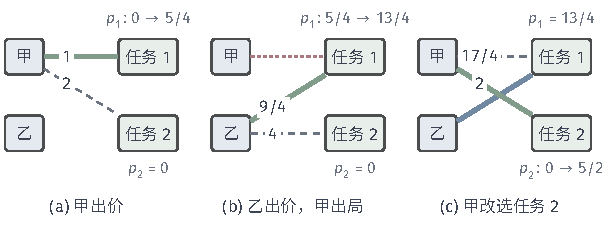
\includegraphics[width=104.122mm]{figures/01-basic-mathematics/04-graphs/tikz/c3-assign-auction/figure.pdf}
  \caption{Auction算法在成本矩阵$\left[\begin{smallmatrix}1&2\\1&4\end{smallmatrix}\right]$上的三次出价，$\varepsilon=1/4$。边旁为出价时的调整成本$c_{i,j}+p_j$，物品旁为价格变化；绿色为本次所得，蓝色为保留的持有，红色点线为被抢走的持有。}
  \label{fig:graph-opt-auction}
\end{figure}

与KM算法相比，Auction算法不要求所选的边恰好紧，只要求每人手中的物品至多比最好选择差$\varepsilon$。这换来了简单的局部操作，但要回答误差在$r$个人身上怎样累计、何时仍精确最优\scite{math-graph-bertsekas1991linear}。

\subsubsection{算法流程}

\paragraph{算法状态与初始化}
输入是成本矩阵和$\varepsilon>0$，不算状态。手工竞价的四份记录对应以下状态：
\begin{itemize}
  \item 价格$p_j$：初值全为$0$。
  \item 物品持有者$\mathrm{owner}(j)$与竞标者所得$\sigma(i)$：两套互相对应的记录，初值全为空。
  \item 未指派者队列$Q$：初值含全部竞标者。
\end{itemize}
一次出价可能只是把物品从一人转给另一人，已指派的人数不变，所以停止条件看队列是否为空，而不看已经处理了多少人。每次只处理一名未指派者；最小值并列时取编号最小的物品。

\paragraph{竞价、易主与停止}
从队列取出竞标者$i$后，一次出价分三步：
\begin{itemize}
  \item 比较：扫描第$i$行，计算$q_j=c_{i,j}+p_j$，求最小值$q_{(1)}$及物品$j^\star$，再求$q_{(2)}=\min_{j\neq j^\star}q_j$。不同物品并列时$q_{(2)}=q_{(1)}$，涨价恰为$\varepsilon$。
  \item 涨价：$p_{j^\star}\gets p_{j^\star}+q_{(2)}-q_{(1)}+\varepsilon$。
  \item 易主：若$j^\star$已有持有者$k$，置$\sigma(k)$为空并把$k$放回队列；再置$\mathrm{owner}(j^\star)=i$、$\sigma(i)=j^\star$。物品一旦有了持有者，此后始终有持有者。
\end{itemize}
队列为空时，每个竞标者都持有不同的物品，停止并输出指派$\sigma$、原始成本$C(\sigma)$和最终价格。

\begin{algorithm}[Auction算法]
\label{alg:graph-opt-auction}
输入：$r\geq2$阶有限成本矩阵$\bm C$，$\varepsilon>0$。输出：完整指派$\sigma$、原始成本与价格$\bm p$。
\begin{enumerate}
  \item 置$p_j=0$，$\mathrm{owner}(j)$与$\sigma(i)$全为空，全部竞标者入队$Q$。
  \item 若$Q$为空，转第5步；否则取出$i$，对每个$j$计算$q_j=c_{i,j}+p_j$，求$q_{(1)}=\min_jq_j$及取到它的物品$j^\star$，以及$q_{(2)}=\min_{j\neq j^\star}q_j$。
  \item 置$p_{j^\star}\gets p_{j^\star}+q_{(2)}-q_{(1)}+\varepsilon$。
  \item 若$k=\mathrm{owner}(j^\star)$非空，置$\sigma(k)$为空并把$k$加入$Q$。置$\mathrm{owner}(j^\star)=i$、$\sigma(i)=j^\star$，回到第2步。
  \item 输出$\sigma$、$C(\sigma)=\sum_ic_{i,\sigma(i)}$与$\bm p$。
\end{enumerate}
\end{algorithm}

\paragraph{运行示例}
取$\varepsilon=1/4$，初始队列为甲、乙。三次出价都是伪代码第2—4步的同一循环，见表~\ref{tab:graph-opt-auction-trace}：
\begin{itemize}
  \item 甲：选任务$1$，涨价$2-1+1/4=5/4$。
  \item 乙：选任务$1$，涨价$2$，价格变为$13/4$；甲失去任务$1$，重新入队。
  \item 甲：选任务$2$，涨价$17/4-2+1/4=5/2$，队列变空。
\end{itemize}
最终甲配任务$2$、乙配任务$1$，原始成本为$2+1=3$。逐人核对：甲手中物品的调整成本是$2+5/2=9/2$，当前最好选择是$\min\{17/4,9/2\}=17/4$，恰好差$1/4$；乙手中的任务$1$调整成本为$17/4$，另一项为$4+5/2=13/2$，乙持有的就是最好选择。最终价格不是原问题的额外支出。

\begin{table}[!htb]
  \centering\small
  \caption{Auction算法在成本矩阵$\left[\begin{smallmatrix}1&2\\1&4\end{smallmatrix}\right]$上的出价，$\varepsilon=1/4$。比较值为出价时的$c_{i,j}+p_j$；价格与持有者为出价后的状态。}
  \label{tab:graph-opt-auction-trace}
  \begin{tabular}{@{}llllll@{}}
    \toprule
    出价者 & 比较值 & 所选 & 涨价 & 价格$\bm p$ & 持有者 \\
    \midrule
    甲 & $1$，$2$ & 任务$1$ & $5/4$ & $(5/4,0)$ & 甲，— \\
    乙 & $9/4$，$4$ & 任务$1$ & $2$ & $(13/4,0)$ & 乙，— \\
    甲 & $17/4$，$2$ & 任务$2$ & $5/2$ & $(13/4,5/2)$ & 乙，甲 \\
    \bottomrule
  \end{tabular}
\end{table}

\subsubsection{正确性与复杂度}

运行示例结束时，甲的选择比最好选择差$1/4$，乙没有差额。把这项性质一般化，就是算法维护的条件。

\begin{definition}[$\varepsilon$互补松弛]
\label{def:graph-opt-eps-cs}
设$\varepsilon\geq0$，$\bm p$为价格，$\sigma$为部分或完整指派。若每个已指派的竞标者$i$都满足
\[
  c_{i,\sigma(i)}+p_{\sigma(i)}\leq\min_{j}\bigl(c_{i,j}+p_j\bigr)+\varepsilon,
\]
就称$(\sigma,\bm p)$满足\term{$\varepsilon$互补松弛}（$\varepsilon$-complementary slackness）。
\end{definition}

$\varepsilon=0$时，它就是“匹配边是紧边”的价格写法，下面的定理说明这一对应。

\begin{lemma}[$\varepsilon$互补松弛的保持]
初始状态满足$\varepsilon$互补松弛，此后每次出价都保持它。
\end{lemma}

\begin{proof}
初始时没有人被指派，条件自动成立。考虑竞标者$i$对$j^\star$的一次出价。对新持有者$i$，涨价后$c_{i,j^\star}+p_{j^\star}=q_{(2)}+\varepsilon$，而其他物品的调整成本都不小于$q_{(2)}$，$j^\star$本身的调整成本也不小于$q_{(2)}+\varepsilon$，所以条件成立。对其他仍持有物品的竞标者$k$，只有$p_{j^\star}$变了，而$k$持有的不是$j^\star$：$k$手中物品的调整成本不变，右端的最小值不会下降，条件继续成立。失去$j^\star$的人回到未指派状态，不受条件约束。
\end{proof}

\begin{theorem}[Auction算法的误差界]
\label{thm:graph-opt-auction}
设成本矩阵完整有限，Auction算法以完整指派$\sigma$和价格$\bm p$停止，$C^\star$为最优指派成本。则
\[
  0\leq C(\sigma)-C^\star\leq r\varepsilon.
\]
若全部成本为整数且$0<\varepsilon<1/r$，则$\sigma$是最优指派。
\end{theorem}

\begin{proof}
令$u_i=\min_j(c_{i,j}+p_j)$、$v_j=-p_j$。对任意$i,j$有$u_i\leq c_{i,j}+p_j$，即$u_i+v_j\leq c_{i,j}$，所以$(\bm u,\bm v)$是可行标号，由第~\ref{sec:graph-opt-assign-labels}节，$\sum_iu_i+\sum_jv_j\leq C^\star$。由$\varepsilon$互补松弛，$c_{i,\sigma(i)}\leq u_i-p_{\sigma(i)}+\varepsilon=u_i+v_{\sigma(i)}+\varepsilon$，即每条匹配边的剩余量至多为$\varepsilon$。对$i$求和，$\sigma$是置换，每个$v_j$恰出现一次，
\[
  C(\sigma)\leq\sum_iu_i+\sum_jv_j+r\varepsilon\leq C^\star+r\varepsilon.
\]
$C(\sigma)\geq C^\star$是最优值的定义。成本为整数时，$C(\sigma)-C^\star$是小于$r\varepsilon<1$的非负整数，只能为$0$。
\end{proof}

一般的实数成本在固定的正$\varepsilon$下只有这个误差界。两人例中$r\varepsilon=1/2<1$，成本为整数，所以得到的成本$3$精确最优。

有限终止要用到“完整有限成本”和“零初始价格”。记$\Delta=\max_{i,j}c_{i,j}-\min_{i,j}c_{i,j}$。物品一旦被出价就始终有持有者，已持有物品的数目等于已指派的人数；只要还没停止，就至少有一个物品从未被出价，价格仍为$0$。竞标者$i$对$j^\star$出价时，若另有从未被出价的物品$j_0\neq j^\star$，则$q_{(2)}\leq c_{i,j_0}$，涨价后
\[
  p_{j^\star}=q_{(2)}+\varepsilon-c_{i,j^\star}\leq c_{i,j_0}-c_{i,j^\star}+\varepsilon\leq\Delta+\varepsilon.
\]
若没有这样的$j_0$，$j^\star$就是最后一个未被出价的物品，这次出价后人人都有物品，算法停止。每次出价至少涨价$\varepsilon$，同一物品被出价$k$次后价格至少为$k\varepsilon$，所以除停止前的最后一次外，每个物品至多被出价$\Delta/\varepsilon+1$次，总出价次数
\[
  B\leq r\bigl(\Delta/\varepsilon+1\bigr)+1.
\]
这个论证依赖每个物品都可选：禁配实例若不可行，价格可以无限上涨而永不停止。

按总出价次数$B$分析稠密实现：每次出价扫描一行为$O(r)$，读入矩阵为$O(r^2)$，总时间$O(r^2+rB)$；价格、持有者、指派与队列为$O(r)$，成本表另占$O(r^2)$。由上面的界，整数成本且取$\varepsilon=1/(r+1)$时，$B=O(r^2\Delta)$，总时间为$O(r^3\Delta)$，随成本范围增长，不能把KM算法的$O(r^3)$直接套用到Auction算法上。$\varepsilon$越小，误差界越紧，但需要的出价可能越多；更强的复杂度界依赖下一小节的缩放策略\scite{math-graph-bertsekas2025auction-ch2}。

\subsubsection{误差缩放与适用边界}

固定一个很小的$\varepsilon$，开始阶段价格从零慢慢上涨，许多出价只是一点点地挪动价格。\term{$\varepsilon$缩放}（$\varepsilon$-scaling）先用较大的$\varepsilon$完成一个较粗的指派，得到大致合理的价格，再逐阶段缩小$\varepsilon$，并把上一阶段的价格作为下一阶段的初值。教学上最简单的做法是每阶段保留价格、清空指派、全部竞标者重新入队竞价；若想保留部分配对，须先解除不满足新$\varepsilon$条件的配对再继续。只缩小参数而保留完整指派是错误的：队列已空，算法会直接停止，新的$\varepsilon$条件根本没有被检查。最后一阶段的$\varepsilon$按定理~\ref{thm:graph-opt-auction}的要求选取\scite{math-graph-bertsekas2024auction}。

非方阵、未分配惩罚等情形，先按第~\ref{sec:graph-opt-assign-rectangular}节补成方阵。允许边不完整时，竞标者只在自己的允许物品中比较，这时要先用第~\ref{sec:graph-opt-match-algorithm}节的方法确认存在完美匹配，因为基本算法不会自行识别不可行。只有一个允许物品的行，排除最好选择后没有次好值，涨价公式无法使用；这样的行在任何完整指派中都只能配这个物品，可以先把这一对固定下来，删去相应的行和列。不能把不存在的次好值当成$+\infty$代入公式，那会让价格变成无穷。

浮点实现中，涨价、并列判断和$\varepsilon$条件都受舍入影响，$\varepsilon$很小时涨价可能被舍入吞掉一部分。整数成本下“$\varepsilon<1/r$即精确最优”的结论，要求算术精度足以区分相差$\varepsilon$的值。并行和异步竞价要处理同时争抢的冲突，可作为后续阅读，其复杂度结论不能搬到本节的串行版本。

\subsection{方法比较与结果检验}
\label{sec:graph-opt-assign-analysis}

两种算法解同一个方阵指派。KM算法保持可行标号、只在紧边上增广，结束时给出精确证书，可直接处理禁配，稠密方阵上为$O(r^3)$。Auction算法维护价格和满足$\varepsilon$互补松弛的部分指派，每步一次出价和易主；其保证随$\varepsilon$、成本整数性和算术精度而定，出价次数随成本范围与$\varepsilon$变化，比较前须先说明这些条件。

检验指派先看原始问题的可行性：每个真实对象按模型要求配对或计入惩罚，所用的列互不相同，全部配对都是允许边；再按原始成本重算总成本。KM算法的结果还要检查证书：对全部允许边验证$u_i+v_j\leq c_{i,j}$，对所选的边验证取等号，并核对总成本等于$\sum_iu_i+\sum_jv_j$。在两人例中，四条边的剩余量依次为$0,0,0,2$，所选的甲—$2$、乙—$1$剩余量为零，成本与下界同为$3$。Auction算法的结果检查最终价格下每人的$\varepsilon$互补松弛，再由定理~\ref{thm:graph-opt-auction}给出目标误差界；只有在整数成本与$\varepsilon<1/r$等条件下才能称为精确最优。浮点实现中，可行性、紧性和出价比较都只能在容差内判断，应说明所用容差，不把近似相等当成精确证书。

标号和价格都在为配对成本提供可以核查的界：可行标号直接给出下界，价格经$u_i=\min_j(c_{i,j}+p_j)$、$v_j=-p_j$转成同样的下界。第~\ref{sec:graph-min-cost-flow}节把这种给顶点配数的做法推广到一般容量与供需网络上的节点势；指派也能写成那里的特例，但统一的模型并不意味着必须选用相同的算法。
